\documentclass[acmlarge]{acmart}
%%
%% \BibTeX command to typeset BibTeX logo in the docs
\AtBeginDocument{%
  \providecommand\BibTeX{{%
    Bib\TeX}}}

\usepackage{subcaption}

%% Rights management information.  This information is sent to you
%% when you complete the rights form.  These commands have SAMPLE
%% values in them; it is your responsibility as an author to replace
%% the commands and values with those provided to you when you
%% complete the rights form.
\setcopyright{acmlicensed}
\copyrightyear{2026}
%\acmYear{2026}
%\acmDOI{XXXXXXX.XXXXXXX}

%% These commands are for a JOURNAL article.
%\acmJournal{POMACS}
%\acmVolume{X}
%\acmNumber{X}
%\acmArticle{XXX}
%\acmMonth{X}

%%
%% Submission ID.
%% Use this when submitting an article to a sponsored event. You'll
%% receive a unique submission ID from the organizers
%% of the event, and this ID should be used as the parameter to this command.
%%\acmSubmissionID{123-A56-BU3}


%%
%% end of the preamble, start of the body of the document source.
\begin{document}

%%
%% The "title" command has an optional parameter,
%% allowing the author to define a "short title" to be used in page headers.
\title{Junkyard Benchmarking: Assessing Repurposed Smartphone Cluster Performance in Academic Usecases}

%%
%% The "author" command and its associated commands are used to define
%% the authors and their affiliations.
%% Of note is the shared affiliation of the first two authors, and the
%% "authornote" and "authornotemark" commands
%% used to denote shared contribution to the research.
\author{Abas Mohamed}
\email{aam037@ucsd.edu}
\authornote{All authors contributed equally to this research.}
%%\orcid{1234-5678-9012}
%%\author{G.K.M. Tobin}
%%\correspondingauthor
%%\email{webmaster@marysville-ohio.com}
\affiliation{%
  \institution{University of California, San Diego}
  \city{La Jolla}
  \state{California}
  \country{USA}
}

\author{Ayushmaan Puri}
\authornotemark[1]
\affiliation{%
  \institution{University of California, San Diego}
  \city{La Jolla}
  \state{California}
  \country{USA}}
\email{aypuri@ucsd.edu}

\author{Richard Vo}
\authornotemark[1]
\affiliation{%
  \institution{University of California, San Diego}
  \city{La Jolla}
  \state{California}
  \country{USA}}
\email{rivo@ucsd.edu}

\author{Shuzheng Zhang}
\authornotemark[1]
\orcid{0009-0001-9438-7685}
\affiliation{%
  \institution{University of California, San Diego}
  \city{La Jolla}
  \state{California}
  \country{USA}}
\email{shz078@ucsd.edu}


%%
%% By default, the full list of authors will be used in the page
%% headers. Often, this list is too long, and will overlap
%% other information printed in the page headers. This command allows
%% the author to define a more concise list
%% of authors' names for this purpose.
%\renewcommand{\shortauthors}{Trovato et al.}

%%
%% The abstract is a short summary of the work to be presented in the
%% article.
\begin{abstract}

The Junkyard Project \cite{10.1145/3575693.3575710} aims to repurpose old and unusable smartphones as compute units for distributed computing \cite{switzer2025hardware}. One target use case is academic autograding; in the most recent offering of \textit{Intro to Parallel Computing}, 330 students shared just 40 GPU nodes on DSMLP\footnote{UCSD's Data Science and Machine Learning Platform}, and demand routinely spiked around deadlines. Student submissions don't need raw GPU power; they need a consistent, available execution environment. Repurposed smartphones fit perfectly: power-efficient, self-contained, standardized, and sourceable at near-zero cost. A dedicated phone cluster eliminates competition for shared HPC resources. This project results in a pipeline that will estimate how many phones are needed to serve a class of $n$ students without meaningful queuing delays.

\end{abstract}

\begin{CCSXML}
<ccs2012>
   <concept>
       <concept_id>10010405.10010489.10010490</concept_id>
       <concept_desc>Applied computing~Computer-assisted instruction</concept_desc>
       <concept_significance>500</concept_significance>
       </concept>
   <concept>
       <concept_id>10002944.10011123.10011674</concept_id>
       <concept_desc>General and reference~Performance</concept_desc>
       <concept_significance>500</concept_significance>
       </concept>
   <concept>
       <concept_id>10003033.10003079.10003080</concept_id>
       <concept_desc>Networks~Network performance modeling</concept_desc>
       <concept_significance>300</concept_significance>
       </concept>
   <concept>
       <concept_id>10010405.10010489.10010491</concept_id>
       <concept_desc>Applied computing~Interactive learning environments</concept_desc>
       <concept_significance>300</concept_significance>
       </concept>
   <concept>
       <concept_id>10010147.10010341.10010349.10010360</concept_id>
       <concept_desc>Computing methodologies~Interactive simulation</concept_desc>
       <concept_significance>500</concept_significance>
       </concept>
 </ccs2012>
\end{CCSXML}

\ccsdesc[500]{Applied computing~Computer-assisted instruction}
\ccsdesc[500]{General and reference~Performance}
\ccsdesc[300]{Networks~Network performance modeling}
\ccsdesc[300]{Applied computing~Interactive learning environments}
\ccsdesc[500]{Computing methodologies~Interactive simulation}


%\received{20 February 2007}
%\received[revised]{12 March 2009}
%\received[accepted]{5 June 2009}

%%
%% This command processes the author and affiliation and title
%% information and builds the first part of the formatted document.
\maketitle


\section{Project Introduction}

Modern computer science education increasingly depends on shared
high-performance computing (HPC) infrastructure. Universities pool GPU
and CPU resources into shared clusters, giving students access to
hardware they could not otherwise afford and enabling courses to assign
computationally intensive work at scale. University-operated HPC
systems are, however, significantly under-resourced relative to
industry and national laboratories, and during
peak demand researchers and students alike face long wait times that
slow iteration-heavy workflows~\cite{hpcsurvey2025}. These pressures
are most acute in instructional settings, where deadline-driven
submission patterns cause demand to spike sharply and unpredictably.

In a recent offering of Intro to Parallel Computing at UC San Diego,
330 students shared just 40 reservable GPU nodes on the campus DSMLP
cluster. During low-traffic periods the allocation was adequate.
Around assignment deadlines, queues grew long enough to delay feedback
by hours. This reflects a broader structural mismatch between
shared, general-purpose compute and the highly variable demand
patterns of large programming courses.

Automated grading systems---autograders---are now a standard tool for
managing courses at this scale. They provide immediate, consistent
feedback without requiring large instructional teams, and make it
practical to run larger courses~\cite{keuning2018}. More frequent
engagement with autograder feedback is also associated with improved
student outcomes~\cite{tran2025}. But autograders are only as
effective as the infrastructure running them. If the execution
environment is shared with other workloads, availability becomes inconsistent, and the feedback loop breaks down precisely when students need it most.

Critically, student submissions for an introductory parallel computing
course do not require high-end GPU throughput. They need a standardized
execution environment that returns consistent, reproducible results
quickly. A cluster of repurposed smartphones can provide exactly this,
at a fraction of the cost of purpose-built server hardware and without
competing for shared HPC allocations.

The case for smartphone-based clusters is well established in prior work. Ranganathan et al.\ demonstrated the feasibility of running automated academic grading on a repurposed phone cluster, showing that even a four-phone cluster can process 33 grading tasks per minute~\cite{ranganathan2025junkyard}. Switzer et al.\ showed more broadly that such clusters are between 9.8$\times$ and 18.9$\times$ more carbon efficient than equivalent cloud instances~\cite{10.1145/3575693.3575710}. Ngoy et al.\ further showed that e-waste smartphones can be repurposed as small-scale data centers capable of efficiently processing and storing data~\cite{ngoy2025ewaste}. Beyond computational performance, the environmental case is compelling on its own: the WEEE Forum and UNITAR estimate that in 2022 alone, roughly 5.3 billion mobile phones were discarded globally, the vast majority destined for landfills or incineration despite remaining functionally intact~\cite{weeeforum2022}. Redirecting even a small fraction of these devices into educational infrastructure extends their useful life and offsets demand for newly manufactured hardware.

Smartphones are not without challenges as compute nodes. They are designed for battery-operated consumer use, and their aggressive power governors throttle CPU and GPU frequency under sustained load, making consistent performance harder to fully guarantee. Flashing a standard Linux distribution to replace the stock OS is a prerequisite for cluster-grade control, and the process is device-specific and labor-intensive. That said, their standardized hardware profiles make execution environments reproduible across nodes once deployed, and their ubiquity means institutions can source them at little to no cost. For the autograding use case specifically, were worloads are short-lived and latency tolerance is moderate, these tradeoffs are acceptable. A dedicated phone cluster still offers a meaningfull improvement over competing for slots on an oversubscribed shared HPC system.

This paper investigates how many phones are needed to serve a class of $n$ students without meaningful queuing delays, and presents a principled estimation strategy grounded in real submission data from a recent course offering.

\section{Related Works}
 
\subsection{Smartphone Repurposing for Distributed Computing}

Early work established the basic feasibility of mobile hardware as distributed compute nodes. Büsching et al.\ built a six-node Android cluster running LINPACK benchmarks via MPI, showing smartphone compute capacity was comparable to workstation-class hardware of the same era~\cite{busching2012droidcluster}. Arslan et al.\ developed CWC, a scheduling framework that achieved 1.6$\times$ faster task completion by exploiting charging idle time~\cite{arslan2015cwc}. Sanches proposed a mobile device cloud using a move-computation-to-data strategy to minimize inter-device data exchange~\cite{sanches2017distributed}. These systems, however, used temporarily idle consumer devices rather than dedicated repurposed hardware. Switzer et al.\ addressed this directly, building a cloudlet of repurposed Pixel~3A phones and introducing the Computational Carbon Intensity metric to quantify the carbon efficiency of extending device lifetimes. Their clusters were 9.8$\times$--18.9$\times$ more carbon efficient than equivalent AWS EC2 instances~\cite{10.1145/3575693.3575710}, a finding Switzer's dissertation extended to a broader class of repurposed hardware~\cite{switzer2025hardware}. Ranganathan et al.\ built on this platform, deploying Kubernetes and Docker on a 16-phone Pixel Fold cluster for serverless autograding and computer vision inference~\cite{ranganathan2025junkyard}. Ngoy et al.\ independently demonstrated e-waste smartphones as small-scale data centers, achievable at roughly 8 euros per device~\cite{ngoy2025ewaste}.
 
\subsection{Autograding Infrastructure}
 
Automated grading systems have become standard in large programming
courses. Keuning et al.\ conducted a systematic literature review of
101 autograding tools, finding that most provide fully automated
assessment with near-instantaneous feedback and support for multiple
resubmissions~\cite{keuning2018}. Their review established that
immediate feedback and consistent evaluation criteria are the primary
drivers of student satisfaction and learning outcomes. Zhang et al.\
extended this empirical picture with an observational study across five
community colleges, finding that students who check autograder feedback
more frequently achieve measurably higher scores~\cite{tran2025}.
 
\subsection{Shared HPC in Academic Settings}
 
University-operated HPC systems are a critical resource for both
research and instruction, but they remain significantly
under-resourced relative to industry and national laboratory
infrastructure~\cite{hpcsurvey2025}. Institutions such as Stanford,
Columbia, and Georgia Tech maintain shared clusters specifically for
coursework, but allocations are fixed and usage is governed by
policies designed primarily around research workloads rather than the
bursty, deadline-driven patterns of student
submissions~\cite{hpcsurvey2025}. This mismatch is well documented: shared
clusters experience long wait times and degraded throughput precisely
during peak instructional demand~\cite{hpcsurvey2025}. Proposals to
address this have included cloud bursting, priority-based scheduling,
and dedicated instructional partitions, but each introduces either
cost, complexity, or fairness tradeoffs that are difficult to resolve
within a course budget.
 
\subsection{Sustainable Computing and E-Waste}
 
The environmental motivation for hardware repurposing is grounded in
manufacturing carbon, not operational energy. Suckling and Lee's life
cycle analysis of smartphones found that manufacturing dominates
greenhouse gas emissions over the device lifetime, meaning that
extending device life through repurposing yields a substantially better
carbon outcome than recycling or disposal~\cite{suckling2015lifecycle}.
The scale of the problem is significant: the WEEE Forum and UNITAR
estimate that 5.3 billion mobile phones were discarded in 2022 alone,
forming a major fraction of the 62 million tonnes of global e-waste
generated that year~\cite{weeeforum2022}. Despite containing valuable
metals and largely functional compute hardware, the majority of these
devices are hoarded, landfilled, or incinerated. Repurposing programs
that redirect even a small fraction of this stock into productive use
extend device lifetimes, displace new hardware manufacturing, and
reduce the total embodied carbon of a computing deployment.

\section{Project Overview}

We propose a simulator to estimate the number of nodes needed. We are approaching the project in three general areas, as seen in Figure~\ref{fig:project_workflow}:

\begin{itemize}
    \item Student data: Here we collect and analyze the past student data for the course offering, as well as modeling the data so it can be generated to fit a class of any scale.
    \item Performance metrics: Here we benchmark the real clusters and use the results as the basis for our simulator behaviors.
    \item Simulation: Here we generate the submissions to a class of any scale, and run the simulation to get our final results.
\end{itemize}

\begin{figure}[H]
  \centering
 
\includegraphics[width=0.75\linewidth]{final/images/workflow_updated.png}
  \caption{Project Workflow}
  \Description{Project Workflow}
  \label{fig:project_workflow}
\end{figure}

\section{Historic Data and Analysis}

\subsection{CSE 160 Data}

\subsubsection{Data collection}
Collecting data from CSE 160 -  Intro to Parallel Computing at UC San Diego was constrained by two factors: Gradescope (e-grader of choice for this class) does not expose an API for bulk data export \cite{gradescope_guides}, and student submission records are protected under FERPA. One of the members on the team ---Tom (Shuzheng)--- was a part of the instructional staff for the class and therefore had to manually webscrape each programming assignment and anonymize them for the rest of the team to work with.

\subsubsection{Limitations}
Because data collection relied on webscraping Gradescope, we had access only to formal submission records. Interactive development sessions on DSMLP, accessed directly via SSH and independent of Gradescope, were not captured. This means that the data reflects assignment submission load but not the ambient compute demand students generate while iterating on their code. Additionally, the webscraping process aggregated results across all execution targets into a single export: submission times reflect grading runs across x86 CPU, NVIDIA GTX 1080Ti, Qualcomm Adreno 643, and Google Pixel Fold nodes without distinguishing between them.

\subsection{Analysis and Modeling}
\label{sec:gmm}
To characterize student workload patterns, we fit two independent
probabilistic models per programming assignment: one capturing when
submissions arrive over the assignment window, and one capturing how
long submitted jobs take to execute. Both models use Gaussian Mixture
Models (GMMs) selected via the Bayesian Information Criterion (BIC).
All models are fit per assignment.
\subsubsection{Submission Timing Model}
 
Submission timing data was available for all programming assignments.
For each assignment, submission timestamps were converted to hours
elapsed since the first recorded submission, producing a non-negative
scalar for each submission. This parameterization anchors all
assignments to a common relative timeline regardless of absolute
calendar date.
 
We fit a GMM to the resulting distribution of submission hours. The
number of components $k$ was selected by minimizing BIC over the range
$k \in [1,\, \lfloor T/24 \rfloor]$, where $T$ is the total
assignment span in hours, bounding the search to at most one component
per day of the assignment window. Each candidate model was initialized
with ten random restarts (\texttt{n\_init=10}) to reduce sensitivity
to local optima, and trained for up to 500 EM iterations with full
covariance. The resulting mixture takes the form
 
\begin{equation}
    f(t) = \sum_{j=1}^{k} w_j \,\mathcal{N}(t \mid \mu_j,\, \sigma_j^2),
    \label{eq:timing_gmm}
\end{equation}
 
\noindent where $t$ is hours since first submission, and $w_j$,
$\mu_j$, $\sigma_j$ are the weight, mean, and standard deviation of
component $j$, respectively, sorted chronologically by $\mu_j$.
Components correspond naturally to distinct submission bursts, which
we observe to align with the days preceding the assignment deadline.

\begin{figure}[H]
  \centering
  \begin{subfigure}[t]{0.48\linewidth}
    \centering
    
\includegraphics[width=\linewidth]{final/images/gmm_hours_PA7.png}
    \caption{GMM fitted to the submission timing for programming assignment 7}
    \Description{GMM fitted to the submission timing for programming assignment 7}
    \label{fig:gmm_hours}
  \end{subfigure}\hfill
  \begin{subfigure}[t]{0.48\linewidth}
    \centering
    
\includegraphics[width=\linewidth]{final/images/gmm_runtime_PA3.png}
    \caption{GMM fitted to the runtimes of submissions for programming assignment 3}
    \Description{GMM fitted to the runtimes of submissions for programming assignment 3}
    \label{fig:gmm_runtime}
  \end{subfigure}

  \caption{Gaussian mixture model fits for PA7 timing and PA3 runtime.}
  \label{fig:gmm_side_by_side}
\end{figure}

\subsubsection{Job Runtime Model}
 
Runtime data was available for programming assignments 3, 4, 5, 7, and
8, which were evaluated on execution time in addition to correctness.
The remaining assignments were graded for correctness only and
produced no timing measurements.
 
Before fitting, submissions were partitioned into three categories.
Pre-execution failures --- submissions where the grading container
failed before any student code ran --- produced no runtime measurement
and were excluded entirely. Timeouts, recorded as $-1$ in the dataset,
represent submissions that either exceeded the grader's kill window or
failed to secure an execution node on DSMLP during the Gradescope
handoff; these were excluded from the GMM fit but their frequency was
tracked separately as a timeout fraction $\phi$ of all executed
submissions. The remaining valid runtimes formed the fitting population.
 
Runtime distributions in this setting are right-skewed and span
several orders of magnitude, reflecting the diversity of student
implementations. We therefore log-transformed valid runtimes prior to
fitting, modeling $\log(\text{runtime}_{\text{ms}})$ as a Gaussian
mixture, which is equivalent to modeling the original runtimes as a
mixture of log-normals. The component count $k$ was again selected by
BIC, with the search range bounded by the assignment duration in days,
and each candidate model trained with ten restarts and full covariance.
The mixture in log-space is
 
\begin{equation}
    g(x) = \sum_{j=1}^{k} w_j {N}(x \mid \mu_j,\, \sigma_j^2),
    \quad x = \log(\text{runtime}_{\text{ms}}),
    \label{eq:runtime_gmm}
\end{equation}
 
\noindent with components sorted by $\mu_j$ in ascending order.
For each component, the median runtime in the original millisecond
scale is recovered as $\exp(\mu_j)$, and the 5th and 95th percentiles
as $\exp(\mu_j \mp 1.645\,\sigma_j)$.
 
The timeout fraction $\phi$ is reported alongside the GMM parameters
for each assignment. Timeouts impose a distinct load pattern from
ordinary jobs: rather than completing and releasing a worker, they hold
a worker thread for the full duration of the grader kill window,
making their contribution to cluster load disproportionate to their
count.

\section{Submission Generation}
To simulate cluster load without requiring live student traffic, we generate synthetic submission traces by sampling from the fitted GMMs described in the previous section. Each synthetic trace represents a complete assignment submission period for a class of $n$ students. Based on observed behavior in CSE~160, students submit approximately three attempts per assignment on average, so a class of $n$ students produces roughly $3n$ synthetic submissions. For the reference class size of 330 students, this yields approximately 1,000 submissions per assignment.

\subsection{Decoupled Timing and Runtime Sources}
The generator accepts independent PA indices for submission timing and job runtime, allowing the two distributions to be drawn from different assignments. This decoupling is useful when runtime data is unavailable for a given assignment --- recall that only PAs 3, 4, 5, 7, and 8 carry runtime measurements --- and when the goal is to stress-test the cluster under timing patterns from one assignment with runtime characteristics from another. Unless otherwise specified, timing and runtime are drawn from the same assignment.

\subsection{Sampling Procedure}
 
Both GMMs are refit from the filtered data at generation time using the same BIC procedure described in Section~\ref{sec:gmm}. Submission arrival times are drawn by sampling $N$ points from the timing GMM and clipping to $[0, \infty)$ to eliminate the small probability mass that full-covariance Gaussians near $t = 0$ place on negative values. Job runtimes are drawn by sampling $N$ points from the runtime GMM in log-space and exponentiating, yielding samples from the underlying log-normal mixture:
 
\begin{equation}
    \hat{r}_i = \exp\!\left( z_i \right), \quad z_i \sim \sum_{j=1}^{k} w_j \,\mathcal{N}(\mu_j, \sigma_j^2).
    \label{eq:runtime_sample}
\end{equation}
 
\noindent Runtime samples are rounded to the nearest millisecond. Submission scores and active-submission flags are not modeled parametrically. Instead, they are drawn from from the distributions observed in the timing PA's data.
 
Once all fields are sampled, submissions are sorted in ascending order of arrival time to produce a chronological trace. The output is a flat CSV with one row per synthetic submission, containing the attempt index, hours since first submission, runtime in milliseconds, score, and active flag. This trace serves as the input workload for the cluster capacity simulation described in Section~\ref{sec:sim}.

\begin{figure}[h]
  \centering
 
\includegraphics[width=1\linewidth]{final/images/synthetic_comparison.png}
  \caption{Sample data generated for 100, 1000, and 10000 submissions based on PA7's submission rates and PA8's runtimes}
  \Description{Sample data generated for 100, 1000, and 10000 submissions based on PA7's submission rates and PA8's runtimes}
  \label{fig:sample_gen}
\end{figure}
 

\section{Cluster Setup}

We are targeting two existing experimental clusters that we have access to: the Junkyard Cluster known as Strawhat that uses repurposed Google Pixel Fold smartphones with Google Tensor G2 SoC\footnote{System on a Chip}, and a Qualcomm cluster that uses Thundercomm Rubik Pi 3 with Qualcomm Dragonwing QCS6490 SoC. Both clusters are running Kubernetes, and both use ARM smartphone SoCs\footnote{Qualcomm Dragonwing SoC is very similar to their Snapdragon SoCs, which are used by a majority of Android smartphones on the market}, meaning that our tests can be replicated relatively easily between the clusters. Furthermore, the use of both clusters allows us to compare the performance and driver differences between the clusters.

\subsection{Junkyard Strawhat Cluster}

Straw-hat is an x86\_64 Ubuntu 24.04 machine with two network interfaces: one facing the public internet and another one on the internal LAN that all the phones connect to. It runs k3s as the control plane for the main 40-phone cluster, with dnsmasq handling DHCP/DNS for the phones. Straw-hat acts as the jump post that you SSH into, and from there reach the phones over the internal LAN.

The phones themselves are Google Pixel Folds that are perfectly functional with some cosmetic defects that make them unsellable. These are equipped with 8 ARM Cortex CPUs, an ARM Mali G710 GPU, the Google Tensor G2 processor, 12GB of RAM, and 512GB of internal storage.

Preparing the phones requires some labor as Pixel Android (or Pixel UI) comes in the way of flashing them directly. Each phone goes through two flash stages, First, we boot it into fastboot mode, unlock the bootloader (which requires physically confirming on the phone's screen), and flash the stock Google Android factory image. After that, each phone boots into Android briefly so we can enable USB debugging through the developer options menu.

We then flash all partitions and reboot the phone into Debian. Once Debian is running, we connect the USB-C Ethernet adapter to each phone (this allows us to connect to the phone and charge it concurrently). and connect it to the network switch which connects to out jump post, straw-hat. Finally, we run our setup script to assign each phone its unique hostname and format its storage partition.

\subsection{Qualcomm Rubik Pi Cluster}

The Qualcomm cluster as shown in Figure~\ref{fig:qcluster} consists of the main tray with the power supply and the Thundercomm Ribik Pi 3, a managed switch, and a reverse proxy.

\begin{figure}[h]
  \centering
 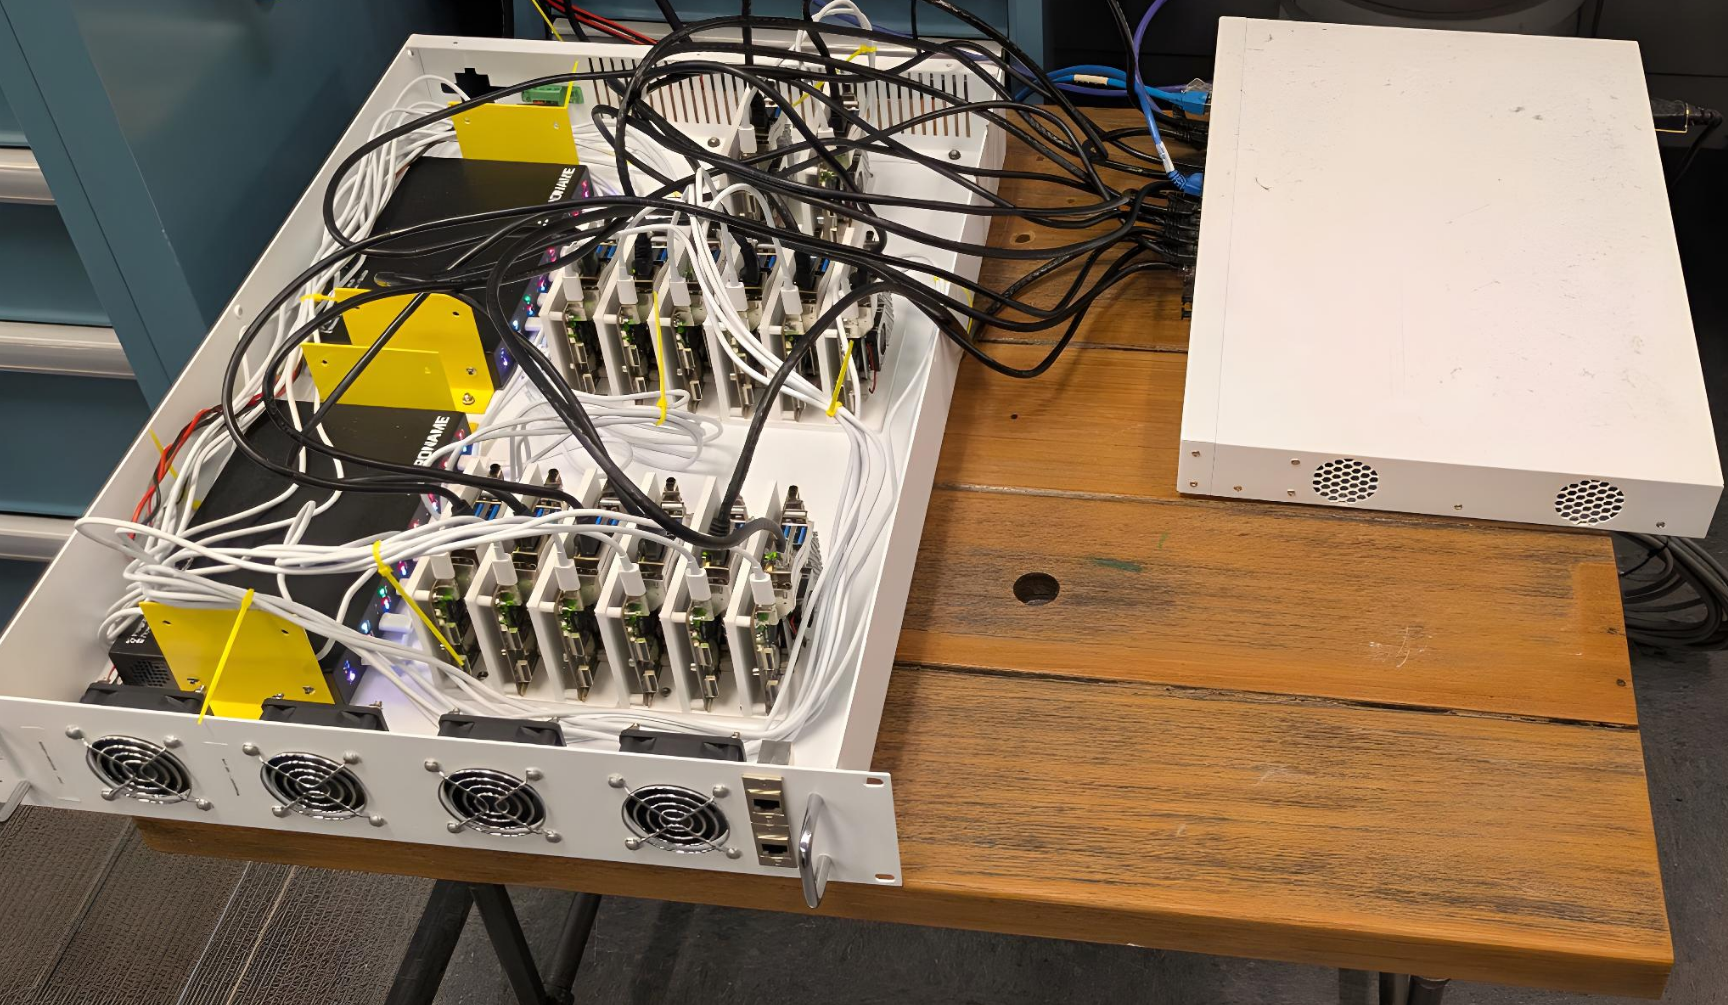
\includegraphics[width=0.7\linewidth]{images/qcluster.png}
  \caption{The current Qualcomm Rubik Pi Cluster setup. The tray with Rubik Pi 3 picture on the left, the switch pictured on the right. Reverse proxy not in picture.}
  \Description{The current Qualcomm Rubik Pi Cluster setup}
  \label{fig:qcluster}
\end{figure}

The main cluster consists of 14 Ribik Pi 3 single board computers equipped with a Qualcomm Dragonwing QCS6490 SoC each, with 8 ARM Kyro 670 CPU cores, an Adreno 630 GPU, 16 GB of onbaord LPDDR5 memory, and a Qualcomm Hexagon NPU\footnote{Neural processing unit}, and gigabit ethernet through a dedicated 8P8C RJ45 port. One of the nodes hosts the Kubernetes Control plane, while the other 13 are worker nodes.

The Rubik Pis are supplied power through a USB PD\footnote{Power Delivery} hub, and run Ubuntu 24.04 through Qualcomm's official flashing software \cite{thundercomm_rubikpi3_docs}. The cluster currently runs MicroK8s, a Kubernetes distribution by Canonical, and can be access by the public internet through a reverse proxy hosted by a x86 machine that is connected to the switch. This is necessary as UCSD does not allow connections directly to the switch. The switch is managed and currently runs pfSense.

A parallel project is in progress concurrently for the Qualcomm cluster to design a custom power delivery system through the GPIO\footnote{General Purpose IO} headers on the boards, and will see a capacity increase as well as an upgrade in the switch used, and see the cluster fit into a standard server rack.

\section{Cluster Metrics}

In order to accurately simulate the cluster, we must first measure its behavior. This is important as it forms the basis of our simulator for any real cluster, and allows us to investigate any behavioral patterns specific to the cluster.

Our method comprises two key components: distributing workloads across clusters and collecting latency measurements at each stage of the auto-grading process. To replicate a real-world grading environment, we used a custom OpenCL workload designed to mirror typical classroom assignments and a scheduler previously used in CSE 160.

We executed multiple test jobs across six nodes, recording timestamps at the following stages, as seen in Figure~\ref{fig:160_workflow} in solid blue:

\begin{enumerate}
    \item Job creation: A host machine from outside of the network assigns a task.
    \item Job receipt: The cluster receives the task.
    \item Cluster processing: The cluster’s autograder server processes the job.
    \item Job queue: The job waits in queue until a node is available and a pod\footnote{A containerized workload in Kubernetes} is created
    \item Execution: The program runs on the assigned node.
    \item Output collection: The program returns its results.
    \item Cleanup: The pod is removed, and the node is reset for the next task.
\end{enumerate}

\begin{figure}[h]
  \centering
 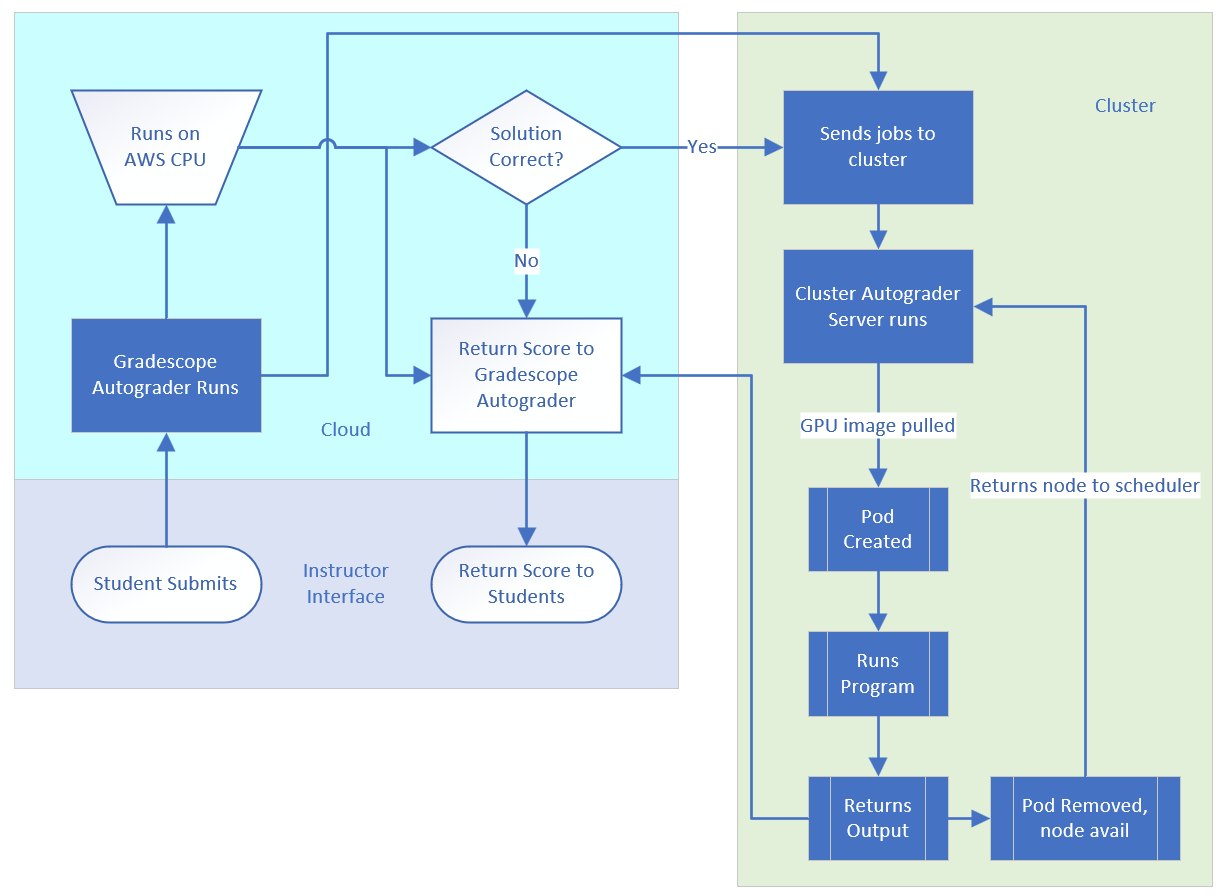
\includegraphics[width=0.6\linewidth]{images/CSE_160_Workflow.png}
  \caption{Workflow for the auto-grading process in CSE 160}
  \Description{Workflow for the auto-grading process in CSE 160}
  \label{fig:160_workflow}
\end{figure}

\subsection{Mock Workload}

To simulate student submissions on the cluster, we developed a mock OpenCL workload that repeatedly performs an FMA-like\footnote{fused multiply-add} operation for a number of iterations until a set runtime is reached. The program then calculates the total number of operations completed and returns the throughput. This allows us to measure the cluster's performance under realistic conditions.

To optimize for hardware capabilities if they are available, we also included the following flags:

\begin{itemize}
    \item \texttt{-cl-fast-relaxed-math}: Enables aggressive mathematical optimizations.
    \item \texttt{-cl-mad-enable}: Activates support for MAD\footnote{multiply-add} instructions.
    \item \texttt{-cl-unsafe-math-optimizations}: Permits non-IEEE-compliant optimizations for faster execution.
\end{itemize}

The workload is intentionally designed to be simple and unoptimized, mirroring the structure of typical student programming assignments in CSE 160. This allows the workload to reflect real-world scenarios, where the student code is usually not very well optimized, and provides more practical metric on system performance.

\subsection{Collecting Cluster Metrics}

In order to collect our metrics, we first needed to complete some initial tasks: modify runner images, configure the Junkyard autograder, deploy the Junkyard autograder, create scripts to benchmark the cluster, and scripts to extract key metrics.

%\begin{figure}[h]
%  \centering
% 
\includegraphics[width=1\linewidth]{final/images/junkyard_latencies.png}
%  \caption{Junkyard Strawhat Cluster Latencies}
%  \Description{Strawhat Cluster Latencies}
%  \label{fig:strawhat-latencies}
%\end{figure}

\begin{figure}[h]
  \centering
 
\includegraphics[width=0.8\linewidth]{final/images/latencies.png}
  \caption{Qualcomm Cluster Latencies}
  \Description{Qualcomm Cluster Latencies}
  \label{fig:qcom-latencies}
\end{figure}

We ended up having to rebuild our runner images alongside configuring the Junkyard autograder for reasons related to the internals of the autograder as well as the CSE160 autograding workflow. While it is not necessary to delve too deeply into the internals of the junkyard autograder, which can be found in \cite{junkyard_autograder,junkyard_project_cse_145}, it is necessary to lay out some relevant implementation details. First, when a submission is made to the deployed Junkyard autograder server, a PA number is passed in as part of the submission. The autograder then schedules a job, where all the job does is spin up a container from our runner image, and then runs a command. Originally, this command called the PA-specific autograding script, as different assignments need to be ran and graded differently. As we only needed to run our mock OpenCL workload, we created our own simple autograding script, and changed the autograder to call that script, leading us to also have to modify our runner image to copy in that autograding script. Second, we also modified the runner images to ensure any dependencies were installed, such as \texttt{opencl-headers}, \texttt{gcc}, \texttt{make}, and etc. Third, we modified the autograder to support a variable-length set of target nodes, using Kubernetes scheduling rules. More specifically, we defined a node affinity with a node selector that matches to any \texttt{kubernetes.io/hostname}--every node has a unique hostname--inside our defined list.

Deploying the reconfigured and rebuilt autograder was straightfoward and just involves following the step-by-step guide inside \cite{junkyard_autograder}. At a high level, deploying the autograder involves the following steps: building the autograder, pushing the built autograder to a GitHub Container Registry (GHCR), creating a server config yaml file, which fortunately was already made for both clusters, tweaking the configuration, and then creating a Kubernetes deployment.

With our autograder up and running, we just needed to start benchmarking and logging each job's output and the aforementioned timestamps. So, we created two main bash scripts, each with nanosecond epoch timestamps, where our main script runs locally and calls the submit script on the cluster, mirroring how "gradescope" typically submits a job to the autograder running on the cluster. We didn't have a public endpoint for the cluster autograders, so we had no choice but to benchmark in such a manner. The submit script also logs the output returned by the workload, which will be used in calculating metrics.

We also created scripts to extract the timestamps, extract the latencies, generate figures such as Figure~\ref{fig:qcom-latencies}, and also calculate our metrics.

Now that everything was setup, we ran benchmarks with different job counts, node counts, and workload times. Figure~\ref{fig:qcom-latencies} showcases one such benchmark run, where one can see the per node jobs that ran, as well as their workload time, their iteration number, as the benchmark script looped through an array of times, and all the different timestamps recorded. We generated figures such as Figure~\ref{fig:qcom-latencies} in order to sanity check the timestamps and thus latencies. However, to collect our final latency data for simulator calibration, we specifically ran a benchmark of $36$ jobs of varying workload times in ${1s, 2s, 4s}$, while targeting $6$ nodes. We ensured that both clusters used the same benchmark setup to uniformly collect latencies.

\subsection{Performance Degradation Model}

To evaluate the performance of a Kubernetes-based cluster accurately, it is essential to measure how its performance changes as the cluster scales. This involves analyzing the impact of increasing node count and job complexity on the control plane, which is a core component of Kubernetes responsible for managing cluster resources. As the number of nodes and concurrent jobs grows, the control plane may experience delays, leading to measurable performance degradation. Additionally, it is critical to confirm that the auto-grading job operates as an \textit{embarrassingly parallel task} — meaning that the workload can be divided into independent subtasks with minimal overhead, ensuring little to no performance loss when parallelization is applied.

\subsubsection{Methodology}

Our approach involves running two sets of jobs with 50 2 second jobs each on the clusters using our mock OpenCL workload to quantify performance implications:

\begin{enumerate}
    \item Baseline Test: Jobs are executed directly on the devices to measure the native throughput. This provides a reference point for comparing the impact of overhead from the Kubernetes infrastructure. We will refer to the resulting native throughput as $\alpha$ for the floating point operations per second, and $A$ for the total floating point operations.
    \item Overhead Test: Jobs are run through the Kubernetes control plane, including intermediate steps like the reverse proxy and the auto-grading server. This setup captures the additional latency introduced by the infrastructure and records timestamps for each stage of the process, and provides us with the overall throughput and performance degradation.
\end{enumerate}

By comparing the results of these two tests, we isolate the effects of the Kubernetes control plane on throughput and can model the performance degradation in our simulator.

\subsubsection{Results}

We calculate the metrics using the following functions over $n$ jobs on $x$ nodes, where FLOPs\footnote{Cumulative Floating-Point Operations} and FLOPS\footnote{Floating-Point Operations Per Second} are the throughput and performance for that job respectively, and $\Delta t$ is the total runtime of the script:

\begin{itemize}
    \item Throughput Excluding Latency: $\tau_{x_i} = \sum_{n}^{} \frac{FLOPS}{n}$
    \item Throughput Including Latency: $\mathrm{T}_{x_i} = \sum_{n}^{} \frac{FLOPs}{\Delta t}$
    \item Efficiency Excluding Latency: $\epsilon_i = \frac{\frac{\tau_{x_i}}{x}}{\alpha}$
    \item Efficiency Including Latency: $\mathrm{E}_i = \frac{\tau_{x_i}}{x} \div \frac{A}{\Delta t}$
    \item Performance Degradation: $\Delta \rho = \tau_{x_i} - \mathrm{T}_{x_i}$
\end{itemize}

Applying these functions yields the performance metric results shown in Figure~\ref{fig:strawhat-metrics} and Figure~\ref{fig:qcluster-metrics}, as well as the performance degradation results shown in Figure~\ref{fig:qcluster_degredation} and Figure~\ref{fig:strawhat_degradation}.

\begin{figure}[h]
  \centering
 
\includegraphics[width=0.75\linewidth]{final/images/strawhat-metrics.png}
  \caption{Junkyard Cluster Metrics}
  \Description{Junkyard Cluster Metrics}
  \label{fig:strawhat-metrics}
\end{figure}

\begin{figure}[h]
  \centering
 
\includegraphics[width=0.75\linewidth]{final/images/qcluster-metrics.png}
  \caption{Qualcomm Cluster Metrics}
  \Description{Qualcomm Cluster Metrics}
  \label{fig:qcluster-metrics}
\end{figure}

Figures ~\ref{fig:strawhat-metrics} and ~\ref{fig:qcluster-metrics} reveal two important trends when validating scability in the clusters. First, the efficiency excluding latency is fairly constant at $100\%$ across both clusters, with a slight deviation due to some random experimental errors. In other words, each node itself suffers negligible performance loss while running the workload in comparison to our baseline. This trend is to be expected, but also necessary, as the only difference between the baseline test and the overhead test, in terms of how the workload is run, is that the overhead test runs the workload inside of a runner docker/container image. Second, and most notably, efficiency including latency sees a large drop across both clusters, even starting from 1 node, but also stays relatively constant as we further scale up, meaning that the latency overhead is a fixed cost that does not scale with the number of nodes. This is key in evaluating scalibility, as we did not wish to see multiple unpredictable drops as we continued scaling up the number of nodes.

Additionally, Figures ~\ref{fig:strawhat-metrics} and ~\ref{fig:qcluster-metrics} reveal interesting differences in the overall performance of the clusters, albeit not related to their scalability factor. It is apparent that the Strawhat cluster has a higher native throughput, which explains the higher throughput when comparing an identical number of nodes between the clusters. However, the actual percentage drop in efficiency due to the latency overhead is around $13\%$ more for the Qualcomm cluster as compared to the Strawhat cluster. One possible contribution to this discrepancy is the reverse proxy that is used for the Qualcomm cluster could be adding on more overhead as compared to the Strawhat cluster. Furthermore, the quality of the network interface controller (NIC) for the Qualcomm cluster could be another contributing factor to a lower effiency including latency.

\begin{figure}[h]
  \centering
 
\includegraphics[width=0.75\linewidth]{final/images/qcluster_degradation.png}
  \caption{Qualcomm Cluster Performance Degradation}
  \Description{Qualcomm Cluster Performance Degradation}
  \label{fig:qcluster_degredation}
\end{figure}

\begin{figure}[h]
  \centering
 
\includegraphics[width=0.75\linewidth]{final/images/strawhat_degradation.png}
  \caption{Strawhat Cluster Performance Degradation}
  \Description{Strawhat Cluster Performance Degradation}
  \label{fig:strawhat_degradation}
\end{figure}

We can see from Figure~\ref{fig:qcluster_degredation} and Figure~\ref{fig:strawhat_degradation} that the performance degradation due to latency scales in an exponential decay model that converges, we can model this with:

$$\gamma \approx -155(1-e^{-1.2x})$$

for the qualcomm cluster, and:

$$\gamma \approx -219(1-e^{-1.08x})$$

for the strawhat cluster.

Because we are already including the latency results from running the auto-grader on 6 nodes in our simulator, and that $\Delta \gamma$, the difference in degradation, is minuscule and within the margin of error, we can safely assume that we do not require a degradation model as the number of nodes increase, and that implementing the numerical overheads alone with suffice.

Note that we did not have access to more than 6 nodes of devices for the junkyard cluster, therefore we can only assume that the performance degradation as seem in Figure~\ref{fig:strawhat_degradation} will exhibit similar behavior to the qualcomm cluster.

\subsubsection{Limitations}

Because the control plane is hosted on a Google Pixel Fold for the Junkyard cluster and a Rubik Pi for the Qualcomm cluster, the network throughput from the control plane to the kubelets\footnote{Kubernetes cluster worker nodes} is limited, and we expect that this connection will saturate as the number of nodes continue to increase. Once it does, we expect to see a sharp decline in the cluster efficiency including overhead, and a dramatic increase in performance degradation. However, we are unable to test this as we are limited by the number of devices we have access to.

\section{Student Interactive Development Sessions}

In a modern university computer science course, a cluster has two primary functions: to support students during development, and to carry out the auto-grading of assignment submissions. We have covered the auto-grading function of the cluster and will now consider its uses when supporting student development. 

\subsection{Background}

Interactive student development sessions allocate a virtual machine on a cluster node so students can write and test code in the exact environment where it will be graded. For a course like CSE 160, where grades depend on runtime after optimization, testing on the precise GPU model is the only reliable way to meet assignment requirements --- driver differences between machines are not cosmetic. CSE 160 attempted to mitigate DSMLP pressure by introducing development containers that students could run locally for correctness checks before submitting for timing. This introduced its own problems: Apple deprecated OpenCL in 2018, forcing course staff to use PoCL\footnote{Portable Computing Language} on macOS, which has implementation differences that cause code to pass locally but fail in the autograder. The feedback loop collapse is also self-reinforcing --- students whose submissions time out resubmit repeatedly while holding their allocated GPU as long as possible, which increases queue pressure for everyone else. A dedicated cluster sized correctly for the course would break this cycle. Generating that size estimate requires session data, which DSMLP does not expose; the following section describes how we derive it from submission records instead.

\subsection{Approach}

We observe that humans have the tendency to complete tasks in bursts, which in this course specifically describes that students tend to work on nothing but their homework before making a submission and letting the auto-grader run. Once they have the results, either they continue working to improve upon it or leave it to come back another time. This is important as it gives us a way to extract development activities from the students from submissions alone.

As an example, Figure~\ref{fig:student_submissions_pa8} is a student’s submission data on PA\footnote{Programming Assignment} 8 in CSE 160. We can see that this student worked on the assignment on March 10th and made two submissions, before pausing and resuming the next day as there is a clear gap between the submissions. The student’s program run-time and score also generally improves as they spend more time on this assignment.

\begin{figure}[h]
  \centering
 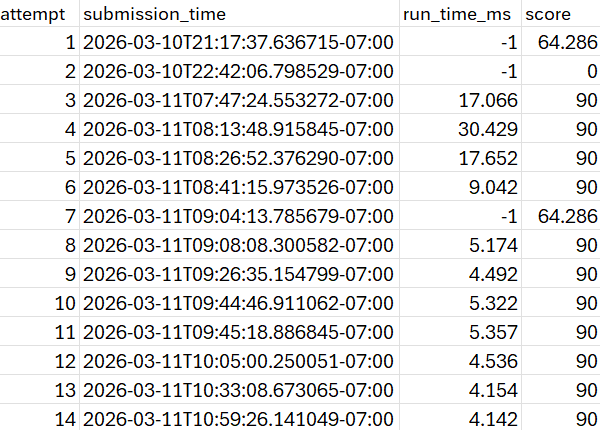
\includegraphics[width=0.4\linewidth]{images/student-submissions.png}
  \caption{A list of one student's submissions for PA8, CSE 160, Winter 2026}
  \Description{A list of one student's submissions for PA8, CSE 160, Winter 2026.}
  \label{fig:student_submissions_pa8}
\end{figure}

As our Gradescope-scraper retrieves the submission data of a student and logs them together, the output will be in order of their attempt, and so we can then safely assign a mock student ID to the student, forming the basis of our analysis as we now have all submissions made by one student.

This type of event is described in \textit{Measuring and modeling bursty human phenomena} \cite{karsai2024measuringmodelingburstyhuman}, which we will be using as the basis for development sessions. A few approaches to detect a burst were described, however, we will simply detect if a submission is inside of a burst by seeing if $\tau$, the time between submissions, is greater than 3 hours, as we have determined it is very unlikely that a student will be continuously working on an assignment if they make no submissions within 3 hours. 

\begin{figure}[h]
  \centering
 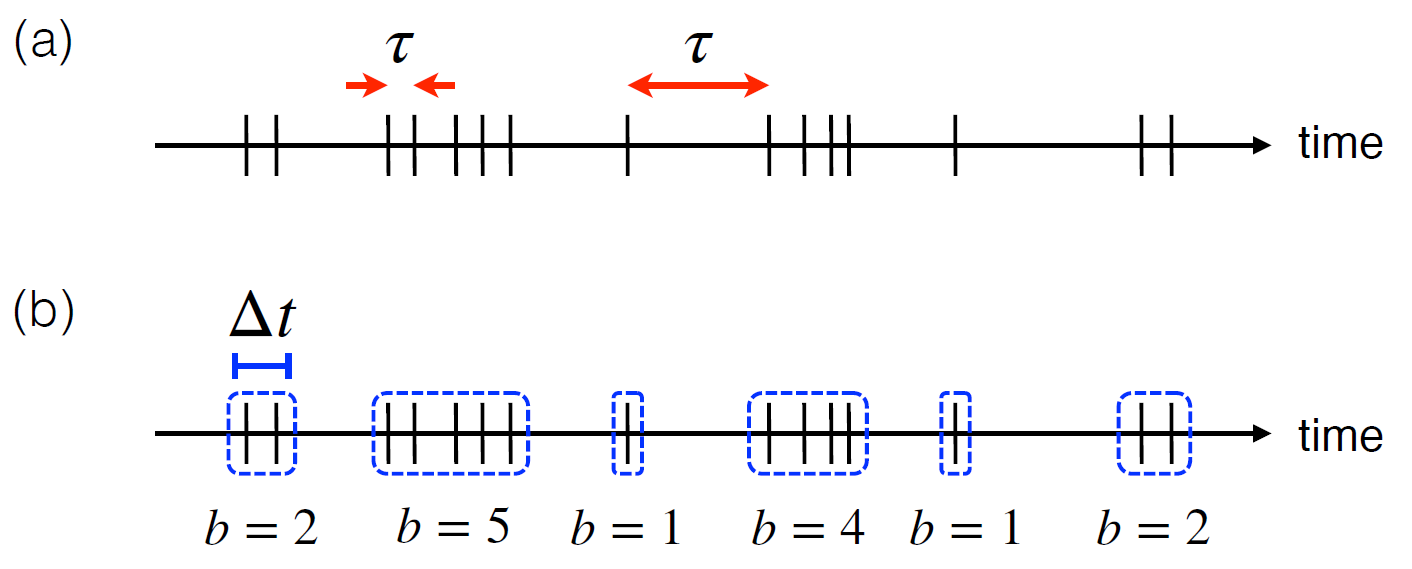
\includegraphics[width=0.5\linewidth]{images/burst-illustration.png}
  \caption{"Schematic diagrams for bursty time series analysis" by Karsai and Jo, used under 
  \href{https://creativecommons.org/licenses/by/4.0/deed.en}{CC BY 4.0}. Unmodified. \cite{karsai2024measuringmodelingburstyhuman}}
  \Description{Schematic diagrams for bursty time series analysis}
  \label{fig:bursty_schematics}
\end{figure}

As shown in Figure~\ref{fig:bursty_schematics}, the submissions are depicted as vertical lines on the time axis, and a burst of submissions depicted as the blue dotted box of time $\Delta t$ is then assigned to them. We will require the following parameters for our generator, which can be changed from the default by the instructor for the specific course and assignment:

\begin{itemize}
  \item $t_{pre} \in \mathbb{Q}^+$: The expected development time before the first submission, modeled with the default Gaussian distribution of $\bar{x}= 3$ hours, $s =$ 1.0
  \item $\tau_{max} \in \mathbb{Q}^+$: The maximum interval between submissions ($\tau$) to be considered as within a burst
  \item $l \in \mathbb{Q}^+$: Randomized lingering time after last submission, modeled with the default Gaussian distribution of $\bar{x}= 0$ hour, $s =$ 0.1
\end{itemize}

We then go through the student's submissions and group them into bursts by $\tau_{max}$, and we now have the discrete array of burst length $\Delta t[n]$ and session start time $x[n]$. We also have the normally generated $t_{pre}[n]$ and $l[n]$ per session, and after combining the parameters, we get the final development sessions for that student:

$$sessions_{a} = \sum_{i=1}^{n} x[i]-t_{pre}[i], lengths_{a}[i] = \Delta t[i] + l[i]$$

Where $a$ is the specific student, $n$ is the number of sessions, and $i$ is one specific session.

\subsection{Limitations}

However, this strategy is severely limited, as we require historic student data as the basis for session generation, making synthetic data incompatible. Furthermore, because we require submissions from individual students, most students do not make enough submissions so that they are statistically significant, and therefore we cannot model and scale the interactive development sessions. It is also not applicable to assignments where the submissions have a rate limit, as it artificially influences the data. Therefore, we can only use this data in our simulator for a class size of the exact number of students that were in CSE 160.

\section{Simulator}
\label{sec:sim}
Through the collection of historical student data and creating the gaussian mixture model. To the gathering of cluster metrics; we have the key components to build our simulator. But the simulator itself can have drawbacks depending on the implementation. What we are proposing in this section is
\begin{itemize}
    \item Student submission only simulator is accurate but not realistic in node count estimation for a classroom. 
    \item Student submission and interactive development session simulator is directly applicable to classroom node count but its backing data has clear limitations as seen previously. 
\end{itemize} 

\subsubsection{Similarities between the two simulators} These two simulators, although encompassing different scopes of classroom node estimation, still share key points. One of these points is how we get the gathered metrics to be inserted into the simulator. In both simulators, there are operations like de-queuing a job off the main queue which has some delay in the real cluster. It would be inefficient to hard-code different cluster metrics in the simulator. Therefore, we take the approach of making a JSON key value pair for each cluster where the simulator will dynamically read in the latencies so it can be applied at runtime as seen in figure \ref{fig:sim_metrics}. Additionally, the simulators also share the pattern of reading in a CSV of the submissions(and sessions for the student submission and interactive development session simulator) which will have the same formats in both. 

\begin{figure}[h]
  \centering
 
\includegraphics[width=.5\linewidth]{final/images/metrics.png}
  \caption{QCluster\footnote{Qualcomm Cluster} metrics that will be injected into the simulator}
  \Description{Json object of the different latencies captured from within qcluster}
  \label{fig:sim_metrics}
\end{figure}

\subsection{Student Submission only Simulator}
Student submissions are handled by the Gradescope platform\cite{gradescope_autograders} that will be routed and sent to the cluster as a submission batch job. The cluster will then run the students program and return the student grade back to Gradescope. 

\subsubsection{Implementation} There is nothing differentiating the batch jobs(student submissions) submitted to the cluster so a single queue(FCFS) for handling job to node assignment will suffice. To prevent submission jobs from waiting in the queue for too long and to match what would occur in a classroom we have a parameter called \textit{TIMEOUT\_MS}. Which is how long a submission will wait in the queue before being dropped. And finally where the simulator does the bulk of the work that can only be done in a simulated environment is find the ideal number of nodes needed to support a class with a drop rate under a threshold. As seen in Figure \ref{fig:submission_sim}, the drop rate target; what we would want to see in a class was set to $<=5 \%$ or 5 percent or less of all jobs can be dropped. 
\begin{figure}[h]
  \centering
 
\includegraphics[width=0.5\linewidth]{final/images/sim.png}
  \caption{Student submission simulator results}
  \Description{Recommended number of nodes given a timeout of 500ms and target droprate of 5 percent}
  \label{fig:submission_sim}
\end{figure}
But a drawback that can be seen from Figure \ref{fig:submission_sim} is that the timeout is very low $500 ms$ or half a second. In a regular classroom setting it would be more realistic to have a submission job timeout in a range around 30 seconds to 1 minute. The reasoning that caused this to happen is that there is little concurrency going on, which results in most submission jobs getting a node quickly. In order to mitigate this and scale it closer to what would appear in the classroom we needed to apply a stricter timeout which yielded a more reasonable node count. Additionally given the environment of CSE 160, students need to run and develop their programs on these virtual machines that have unique drivers. Without development on these virtual machines, errors unrelated to correctness but rather porting would arise. This results in a simulator that only accounts for submission jobs not representing a classroom's behavior accurately where student develop on clusters and submit to the cluster. 

Finally, acknowledging these constraints, we can accurately estimate the node count for a given classroom that only has submission jobs. And even more specifically estimate the node count needed for different assignments as seen in figure \ref{fig:submission_sim_graph}. For two different workload assignments, we can directly look up the nodes needed to support \textit{x} number of students. 
\begin{figure}[h]
  \centering
 
\includegraphics[width=.75\linewidth]{final/images/Class Size vs Nodes Needed.png}
  \caption{Class Size vs Nodes Needed for two different workloads}
  \Description{Recommended number of nodes for x amount of student in a cse 160 class}
  \label{fig:submission_sim_graph}
\end{figure}

\subsection{Student Submission and Interactive Development Session Simulator}
This simulator fixes the weaknesses of the previous simulator by giving more realistic numerical values for the parameters seen in the previous simulator. Such as \textit{TIMEOUT\_MS} changing from half a second to 300,000 milliseconds(5 minutes) as seen in figure \ref{fig:sessions_sim}. That is a much more reasonable number in a classroom. Additionally, it accounts for students developing on the nodes using the session generation method described in section 5. 

\subsubsection{Implementation} When two students, one who wants to get a node for development and one who is trying to submit an assignment to Gradescope, who should get precedence for a node? We answered this from this perspective. Students who lose critical development time cannot get this lost time back. Meaning they may not be able to get the chance to submit. Additionally, submissions would be less attempted since the student who is developing is given adequate chance to develop. And finally submissions can be reattempted. 

To model this behavior, we use a multi-level queue \cite{sattar2014multi} where interactive sessions are given the highest priority and submissions jobs are placed in a lower priority queue. This also has the side affect that interactive development sessions will never be dropped. Students who go over the session limit(6 hours in CSE 160) will be re-queued in the sessions queue and they will not timeout and can wait indefinitely. Since we now have an additional factor to think about in our simulator we must add additional parameters to model this change. So we add two new parameters for the sessions, \textit{SESSION\_WAIT\_TARGET\_MS} which is the amount of time we would want to wait in the queue. Or how long a student may wait to get a node to develop on. And since it is not realistic for all students to hit this target we aim to have \textit{x} percent of the sessions wait $\leq$ our parameter \textit{SESSION\_WAIT\_PERCENTILE}. This can be seen again in our sim from Figure \ref{fig:sessions_sim} where we would want 97 percent of all students to wait under a certain time to get a node to develop on. Finally, our simulator will sweep different numbers of nodes and find the minimum number of nodes that fulfill our parameters. 


\begin{figure}[h]
  \centering
 
\includegraphics[width=.5\linewidth]{final/images/node_count_idev.png}
  \caption{Node count for classroom with student development sessions and gradescope submissions}
  \Description{Recommended number of nodes for x amount of student in a cse 160 class}
  \label{fig:sessions_sim}
\end{figure}

\section{Milestones}

\begin{itemize}
\item \textbf{M0: Project specifications} \\
\textit{Lead: All} \hfill
\textit{Progress: Completed} \\
The document that details project goals and specifics.\\

\item \textbf{M1: Historic Data Collection} \\
\textit{Lead: Tom (FERPA Access required)} \hfill
\textit{Progress: Completed} \\
Historic data from CSE 160 as a baseline for simulations. Rest of the group was blocked till Tom finished scraping and anonymizing the data. \\

\item \textbf{M2: Student Submission Model} \\
\textit{Lead: Ayushmaan and Richard} \hfill
\textit{Progress: Completed} \\
Gaussian Mixture Model based on student submission times and code runtimes. \\

\item \textbf{M2.5: Synthetic OpenCL Workload} \\
\textit{Lead: Tom} \hfill
\textit{Progress: Completed} \\
This milestone was added because we realized we need some sort of program to realistically stress the pixel folds, and also we want to get the throughput data \\

\item \textbf{M3: Virtual Simulator} \\
\textit{Lead: Abas} \hfill
\textit{Progress: Completed} \\
A discrete-event simulator that sweeps pod counts (1 -> N) to find the minimum number of compute pods needed to keep student autograder job timeouts at or below a target drop rate. \\

\item \textbf{M4: Mock Submission Generator} \\
\textit{Lead: Ayushmaan} \hfill
\textit{Progress: Completed} \\
Samples submission times and runtimes to generate a csv file with a desired number of mock submissions.\\
\emph{Milestone modified from Scheduler Integration and Virtual Testing, as original plan was actually in scope with Milestone 3 and merged into it.} \\

\item \textbf{M4.5: Mali Container} \\
\textit{Lead: Tom} \hfill
\textit{Progress: Completed} \\
Build container capable of compiling and running OpenCL programs on the Pixel Folds. \\

\item \textbf{M5: Physical Cluster Validation} \\
\textit{Lead: Ayushmaan, Richard, and Tom} \hfill
\textit{Progress: Completed} \\
Get latencies and throughput of the three available clusters: Strawhat, Qualcomm, and Junkyard. Then, validate results of our simulator by running real-time workloads on the number of nodes given by the simulator. We had to wait for the another group's progress to be able to use qcluster.\\

\item \textbf{M6: Mock interactive development node usage} \\
\textit{Lead: Tom for model, Abas for simulator modifications} \hfill
\textit{Progress: Completed} \\
This milestone was added since we would need some way to model and simulate student interactive development sessions on the nodes based on student submissions, and then generate a list for the simulator.

\item \textbf{M7: Final paper draft} \\
\textit{Lead: All} \hfill
\textit{Progress: Completed}

\item \textbf{M8: Final paper and video} \\
\textit{Lead: All} \hfill
\textit{Progress: Completed}

\end{itemize}
\section{Conclusion}
Re-purposing phones that offer classes compute for student development and auto-grading on GPUs is a task that has clear benefits. However, if students cannot rely on these devices to effectively do their classwork. Then many of the same issues that some students have experienced on other kinds of distributed compute begin to appear again. Junkyard Benchmarking addresses this point by contributing a method to effectively measure the amount of compute needed to support a class. Such that issues like dropped jobs, or a lack of nodes for development can be mitigated. In addition, provide courses with a method to know how much compute they need before even beginning instruction. And this is through our simulator that relies on the GMM and cluster metrics to model the class without having the class present. In future iterations of this project, we may need to collect data on sessions rather than using mock data. And this would allow us to model student behavior more accurately. 

Through benchmarking, we can get a solid idea of how the cluster behaves, which in return tells us what it does well and where it can improve. Junkyard Benchmarking bridges this gap between those who will use the clusters for their everyday tasks such as in CSE 160 and those who develop the cluster. Allowing everyone to yield the full benefits of the cluster.  

\bibliographystyle{ACM-Reference-Format}
\bibliography{references}

\end{document}
\endinput
%%
%% End of file `main.tex'.
